%% LyX 2.3.4.2 created this file.  For more info, see http://www.lyx.org/.
%% Do not edit unless you really know what you are doing.
\documentclass[english,dvipsnames,aspectratio=169,handout]{beamer}
\usepackage{mathptmx}
\usepackage{eulervm}
\usepackage[T1]{fontenc}
\usepackage[latin9]{inputenc}
\usepackage{babel}
\usepackage{amstext}
\usepackage{amssymb}
\usepackage{graphicx}
\usepackage{ifthen}
\usepackage{xcolor}
\usepackage{xspace}
\usepackage{tikz}
\usetikzlibrary{tikzmark}
\usetikzlibrary{calc}
\usepackage{pgfplots}
%\pgfplotsset{compat=1.17}
\usepackage{booktabs}
\usepackage{xpatch}
\usepackage{multirow}
\usepackage{colortbl}
\usepackage{pgfpages}


\xpatchcmd{\itemize}
  {\def\makelabel}
  {\ifnum\@itemdepth=1\relax
     \setlength\itemsep{2ex}% separation for first level
   \else
     \ifnum\@itemdepth=2\relax
       \setlength\itemsep{1ex}% separation for second level
     \else
       \ifnum\@itemdepth=3\relax
         \setlength\itemsep{0.5ex}% separation for third level
   \fi\fi\fi\def\makelabel
  }
 {}
 {}

\ifx\hypersetup\undefined
  \AtBeginDocument{%
    \hypersetup{unicode=true,pdfusetitle,
 bookmarks=true,bookmarksnumbered=false,bookmarksopen=false,
 breaklinks=false,pdfborder={0 0 0},pdfborderstyle={},backref=false,colorlinks=true,
 allcolors=NYUPurple,urlcolor=LightPurple}
  }
\else
  \hypersetup{unicode=true,pdfusetitle,
 bookmarks=true,bookmarksnumbered=false,bookmarksopen=false,
 breaklinks=false,pdfborder={0 0 0},pdfborderstyle={},backref=false,colorlinks=true,
 allcolors=NYUPurple,urlcolor=LightPurple}
\fi

\makeatletter

%%%%%%%%%%%%%%%%%%%%%%%%%%%%%% LyX specific LaTeX commands.
%% Because html converters don't know tabularnewline
\providecommand{\tabularnewline}{\\}

%%%%%%%%%%%%%%%%%%%%%%%%%%%%%% Textclass specific LaTeX commands.
% this default might be overridden by plain title style
\newcommand\makebeamertitle{\frame{\maketitle}}%
% (ERT) argument for the TOC
\AtBeginDocument{%
  \let\origtableofcontents=\tableofcontents
  \def\tableofcontents{\@ifnextchar[{\origtableofcontents}{\gobbletableofcontents}}
  \def\gobbletableofcontents#1{\origtableofcontents}
}

%%%%%%%%%%%%%%%%%%%%%%%%%%%%%% User specified LaTeX commands.
\usetheme{CambridgeUS} 
\beamertemplatenavigationsymbolsempty


% Set Color ==============================
\definecolor{NYUPurple}{RGB}{87,6,140}
\definecolor{LightPurple}{RGB}{165,11,255}


\setbeamercolor{title}{fg=NYUPurple}
\setbeamercolor{frametitle}{fg=NYUPurple}

\setbeamercolor{background canvas}{fg=NYUPurple, bg=white}
\setbeamercolor{background}{fg=black, bg=NYUPurple}

\setbeamercolor{palette primary}{fg=black, bg=gray!30!white}
\setbeamercolor{palette secondary}{fg=black, bg=gray!20!white}
\setbeamercolor{palette tertiary}{fg=gray!20!white, bg=NYUPurple}

\setbeamertemplate{headline}{}
\setbeamerfont{itemize/enumerate body}{}
\setbeamerfont{itemize/enumerate subbody}{size=\normalsize}

\setbeamercolor{parttitle}{fg=NYUPurple}
\setbeamercolor{sectiontitle}{fg=NYUPurple}
\setbeamercolor{sectionname}{fg=NYUPurple}
\setbeamercolor{section page}{fg=NYUPurple}
%\setbeamercolor{description item}{fg=NYUPurple}
%\setbeamercolor{block title}{fg=NYUPurple}

\setbeamertemplate{blocks}[rounded][shadow=false]
\setbeamercolor{block body}{bg=normal text.bg!90!NYUPurple}
\setbeamercolor{block title}{bg=NYUPurple!30, fg=NYUPurple}



\AtBeginSection[]{
  \begin{frame}
  \vfill
  \centering
\setbeamercolor{section title}{fg=NYUPurple}
 \begin{beamercolorbox}[sep=8pt,center,shadow=true,rounded=true]{title}
    \usebeamerfont{title}\usebeamercolor[fg]{title}\insertsectionhead\par%
  \end{beamercolorbox}
  \vfill
  \end{frame}
}

\makeatother

\setlength{\parskip}{\medskipamount} 

\input ../macros

\begin{document}
\input ../rosenberg-macros

%\setbeameroption{show notes on second screen}

\title[DS-GA 1003]{Reduction to Binary Classification}
\author{He He \\
Slides based on Lecture
\href{https://github.com/davidrosenberg/mlcourse/blob/gh-pages/Lectures/09.multiclass.pdf}{09} from David Rosenberg's course materials (\url{https://github.com/davidrosenberg/mlcourse})
}
\date{March 30, 2021}
\institute{CDS, NYU}

\makebeamertitle
\mode<article>{Just in article version}

\section{Overview}
\begin{frame}
{Motivation}
\begin{itemize}
\item So far, most algorithms we've learned are designed for binary classification.
\note[item]{Which ones we've learned can handle more than 2 classes? Multinomial logistic regression, naive Bayes. Next, trees and random forests.}
\item Many real-world problems have more than two classes.
\note[item]{Examples? Text classification, object recognition (ImageNet has more than 20k classes).}
\item<2-> \dis What are some potential issues when we have a large number of classes?
\note<2->[item]{Class imbalance, computation cost for both training and testing, different cost of errors etc.}
\end{itemize}
\end{frame}

\begin{frame}
{Today's lecture}
\begin{itemize}
\item How to \emph{reduce} multiclass classification to binary classification?
\note[item]{Think of binary classification or linear regression as black-box predictors and start from there.}
\item How do we \emph{generalize} binary classification algorithm to the multiclass setting?
\note[item]{What needs to be changed here? The loss function.}
\item Example of very large output space: structured prediction.
\end{itemize}
\end{frame}

\section{Reduction to Binary Classification}
\subsection{Recap: OvA and AvA}
\begin{frame}{One-vs-All / One-vs-Rest}
\begin{description}
    \setlength\itemsep{10pt}
\item<+->[Setting]
\begin{itemize}
\item Input space: $\cx$
\item Output space: $\cy=\left\{ 1,\ldots,k\right\} $
\end{itemize}

\item<+->[Training]
\begin{itemize}
\item Train $k$ binary classifiers, one for each class:
$h_{1},\ldots,h_{k}:\cx\to\reals$.
\item Classifier $h_i$ distinguishes class $i$ (+1) from the rest (-1).
\end{itemize}

\item<+->[Prediction]
\begin{itemize}
\item Majority vote:
\[
h(x)=\argmax_{i\in\left\{ 1,\ldots,k\right\} }h_{i}(x)
\]
\item Ties can be broken arbitrarily.
\end{itemize}
\end{description}
\end{frame}
%

\begin{frame}
{OvA: 3-class example}
\begin{columns}
\begin{column}{0.4\textwidth}
\begin{simpleblock}<1->
{Consider a dataset with three classes:}
\begin{figure}
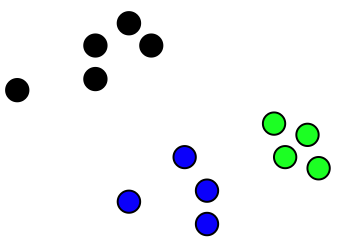
\includegraphics[height=0.25\textheight]{figures/three-class}
\end{figure}
\end{simpleblock}
\end{column}
\begin{column}{0.6\textwidth}
\onslide<3->{
\textbf{Assumption}: each class is linearly separable from the rest.\\
Ideal case: only target class has positive score.
}
\end{column}
\end{columns}

\begin{simpleblock}<2->
{Train OvA classifiers:}
\begin{figure}
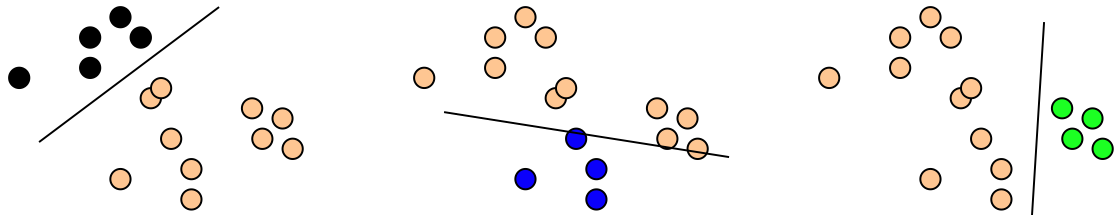
\includegraphics[height=0.25\textheight]{figures/three-class-ova}
\end{figure}
\end{simpleblock}
\note<3->{What's a failure case for OvA?}
\end{frame}

\begin{frame}
{OvA: 4-class non-separable example}
\begin{columns}
\begin{column}{0.4\textwidth}
Consider a dataset with four classes:
\begin{figure}
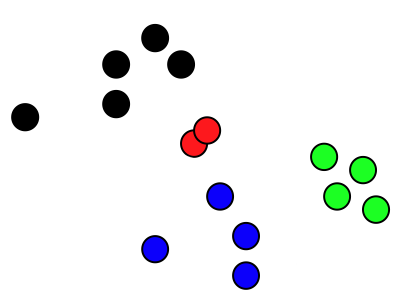
\includegraphics[height=0.25\textheight]{figures/four-class}
\end{figure}
\end{column}
\begin{column}{0.6\textwidth}
\onslide<2->{
Cannot separate \textcolor{red}{red} points from the rest.\\
Which classes might have low accuracy?
}
\note<2->[item]{Blue and green because they are getting positive score from the red classifier.}
\end{column}
\end{columns}

Train OvA classifiers:
\begin{figure}
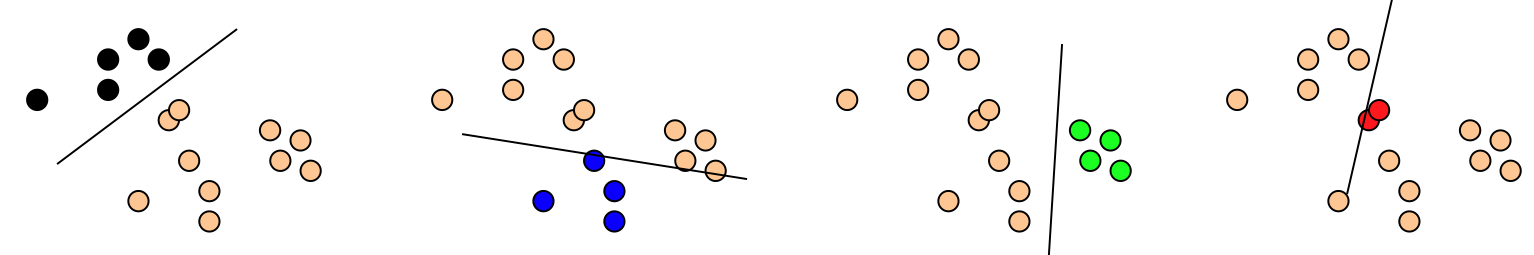
\includegraphics[height=0.25\textheight]{figures/four-class-ova}
\end{figure}
\note<2->[item]{How can we fix this? Note that optimal linear classifiers exist in this example.}
\end{frame}

\begin{frame}
{All vs All / One vs One / All pairs}
\begin{description}
    \setlength\itemsep{10pt}
\item<1->[Setting]
\begin{itemize}
    \setlength\itemsep{2pt}
\item Input space: $\cx$
\item Output space: $\cy=\left\{ 1,\ldots,k\right\} $
\end{itemize}
\note<1>[item]{How many classifiers do we need to train?}

\item<2->[Training]
\begin{itemize}
    \setlength\itemsep{2pt}
\item Train $k \choose 2$ binary classifiers, one for each pair:
$h_{ij}:\cx\to\reals$ $\text{for } i\in [1,k] \text{ and } j\in [i+1, k]$.
\item Classifier $h_{ij}$ distinguishes class $i$ (+1) from class $j$ (-1).
\end{itemize}

\item<3->[Prediction]
\begin{itemize}
    \setlength\itemsep{2pt}
\item Majority vote (each class gets $k-1$ votes)
\[
h(x)=\argmax_{i\in\left\{ 1,\ldots,k\right\} } \sum_{j\neq i}
\underbrace{h_{ij}(x)\1\pc{i<j}}_{\text{class $i$ is +1}} 
- \underbrace{h_{ji}(x)\1\pc{j<i}}_{\text{class $i$ is -1}}
\]
\note<3->[item]{Majority vote: Class $i$ gets a vote each time it is predicted.}
\item Tournament
\note<3->[item]{Tournament: start with random pairs, only winners continue.}
\item Ties can be broken arbitrarily.
\end{itemize}
\end{description}
\end{frame}

\begin{frame}
{AvA: four-class example}
\begin{columns}
\begin{column}{0.4\textwidth}
Consider a dataset with four classes:
\begin{figure}
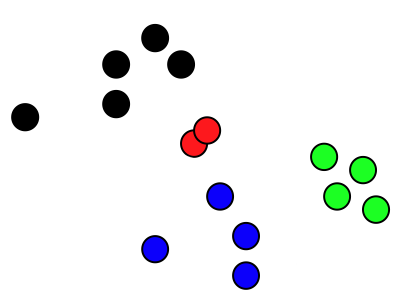
\includegraphics[height=0.25\textheight]{figures/four-class}
\end{figure}
\end{column}
\begin{column}{0.6\textwidth}
\onslide<2->{
\textbf{Assumption}: each pair of classes are linearly separable.\\
More expressive than OvA.
}
\end{column}
\end{columns}

What's the decision region for the red class?
\begin{figure}
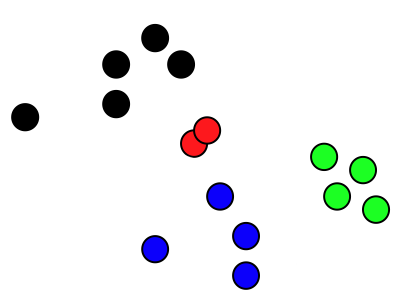
\includegraphics[height=0.3\textheight]{figures/four-class}
\end{figure}
\note<1>[item]{Draw lines separating red from each other classes. The intersection of the three regions get 3 votes (max).}
\end{frame}

\begin{frame}
{\dis OvA vs AvA}
\begin{table}
\begin{tabular}{llcc}

\toprule
& & OvA & AvA \\
\midrule
\multirow{2}{*}{computation} & train & $O(k \onslide<2->{B_{\text{train}}(n)})$ & $O(k^2\onslide<2->{B_{\text{train}}(n/k)})$ \\
                     							   &  test & $O(k\onslide<2->{B_{\text{test}}})$ & $O(k^2 \onslide<2->{B_{\text{test}}})$ \\
       \midrule

\pause
\multirow{3}{*}{challenges}  \pause  & train & class imbalance & small training set \\
                                                   & \multirow{2}{*}{test} & \multicolumn{2}{c}{calibration / scale} \\
                                                    &         &  \multicolumn{2}{c}{tie breaking} \\
\bottomrule

\end{tabular}
\end{table}
Lack theoretical justification but simple to implement and works well in practice (when \# classes is small).

\think{Question}: When would you prefer AvA / OvA? 
\note{If you're using SVM, would you prefer AvA or OvA to save computation?
Dual form would prefer AvA. When number of examples much larger than feature dimensions, dual is more expensive.}
\end{frame}

\subsection{Error correcting output codes}

\begin{frame}
{Code word for labels}
Using the reduction approach, can you train fewer than $k$ binary classifiers?
\pause

\textbf{Key idea}: Encode labels as binary codes and predict the code bits directly.
\pause

OvA encoding:
\begin{table}
\begin{tabular}{|c|c|c|c|c|}
\hline
class & $h_1$ & $h_2$ & $h_3$ & $h_4$ \\
\hline
1 & 1 & 0 & 0 & 0 \\
\hline
2 & 0 & 1 & 0 & 0\\
\hline
3 & 0 & 0 & 1 & 0\\
\hline
4 & 0 & 0 & 0 & 1\\
\hline
\end{tabular}
\end{table}
\pause

OvA uses $k$ bits to encode each label, what's the minimal number of bits you can use?
\end{frame}

\begin{frame}
{Error correcting output codes (ECOC)}
\begin{columns}
\begin{column}{0.4\textwidth}
Example: 8 classes, 6-bit code
\begin{table}
\begin{tabular}{|c|c|c|c|c|c|c|}
\hline
class & $h_1$ & $h_2$ & $h_3$ & $h_4$ &  $h_5$ & $h_6$\\
\hline
1 & 0 & 0 & 0 & 1 & 0 & 0 \\
\hline
2 & 1 & 0 & 0 & 0 & 0 & 0 \\
\hline
\rowcolor{red!20}
3 & 0 & 1 & 1 & 0 & 1 & 0\\
\hline
4 & 1 & 1 & 0 & 0 & 0 & 0 \\
\hline
5 & 1 & 1 & 0 & 0 & 1 & 0 \\
\hline
6 & 0 & 0 & 1 & 1 & 0 & 1 \\
\hline
7 & 0 & 0 & 1 & 0 & 0 & 0 \\
\hline
8 & 0 & 1 & 0 & 1 & 0 & 0 \\
\hline
\end{tabular}
\end{table}
\end{column}
%
\begin{column}{0.6\textwidth}
\begin{description}
\item<1->[Training]
Binary classifier $h_i$: 
\begin{itemize}
\item +1: classes whose $i$-th bit is 1
\item -1: classes whose $i$-th bit is 0
\end{itemize}
\item<2->[Prediction]
Closest label in terms of Hamming distance.
\begin{table}
\begin{tabular}{{|c|c|c|c|c|c|}}
\hline
$h_1$ & $h_2$ & $h_3$ & $h_4$ &  $h_5$ & $h_6$\\
\hline
0 & 1 & 1 & 0 & 1 & 1 \\
\hline
\end{tabular}
\end{table}
\item<3->[Code design]
Want good binary classifiers.
\note<3->[item]{Random or depending on domain knowledge}
\end{description}
\end{column}
\end{columns}
\end{frame}

\begin{frame}
{Error correcting output codes: summary}
\begin{itemize}
\item Computationally more efficient than OvA (a special case of ECOC). Better for large $k$.
\item Why not use the minimal number of bits ($\log_2k$)?
\pause
\begin{itemize}
\item If the minimum Hamming distance between any pair of code word is $d$, then it can correct $\left \lfloor \frac{d-1}{2} \right \rfloor$ errors.
\item In plain words, if rows are far from each other, ECOC is robust to errors.
\end{itemize}
\pause
\item Trade-off between code distance and binary classification performance.
\note<2>[item]{Larger distance -> more binary problems -> more likely to have hard binary problems.}
\item Nice theoretical results \href{http://www.jmlr.org/papers/volume1/allwein00a/allwein00a.pdf}{[Allwein et al., 2000]} (also incoporates AvA).
\end{itemize}
\end{frame}

\begin{frame}
{Review}
Reduction-based approaches:
\begin{itemize}
\item Reducing multiclass classification to binary classification: OvA, AvA, ECOC.
\item Key is to design \textcolor{Green}{``natural'' binary classification} problems without large \textcolor{red}{computation} cost.
\end{itemize}
\pause

But,
\begin{itemize}
\item Unclear how to generalize to extremely large \# of classes.
\item ImageNet: >20k labels; Wikipedia: >1M categories.
\end{itemize}

Next,
generalize previous algorithms to multiclass settings.
\note<2->[item]{What needs to be changed? The loss function.}
\end{frame}

\end{document}
